\subsubsection{Descripción}

El algoritmo a cada paso tiene un camino $P = [v_1 = u, \dots, v_{i-1}]$ e intenta agregar al camino un nuevo nodo $v_i$ de la adyacencia de $v_{i-1}$, hasta que llega al nodo destino $V$. De esta forma recorre todos los caminos entre $U$ y $V$. De entre todos los caminos tales que el peso por $\omega_1$ es menor o igual a K, se guarda el de menor $\omega_2$.

Se implementaron las siguientes podas:

\begin{itemize}
    \item Se exploran solamente caminos simples. Si un camino tiene ciclos, removiéndolo se obtiene uno con menor longitud tanto en $\omega_1$ como en $\omega_2$. Por lo tanto la solución que buscamos no puede tener ciclos, y nos restringimos a caminos simples. La poda se implementó guardando un arreglo que marca para cada nodo si es parte del camino o no. No se agrega nuevamente si ya es parte del camino.
    \item Si el camino parcial $P = [v_1 = u, \dots, v_{i-1}]$ cumple:

        $omega_1(P)$, sumado a la distancia según $\omega_1$ entre $v_{i-1}$ y $V$, es mayor que $K$

entonces se abandona la rama, es decir, no se recorren los caminos que empiezan en $P$, ya que cualquiera de éstos no va a cumplir con la restricción de que $omega_1$ sea menor o igual a $K$.
    \item Si el camino parcial $P = [v_1 = u, \dots, v_{i-1}]$ cumple:

        $omega_2(P)$, sumado a la distancia según $\omega_2$ entre $v_{i-1}$ y $V$, es mayor o igual que el peso según $\omega_2$ del mejor camino encontrado hasta el momento

entonces se abandona la rama, es decir, no se recorren los caminos que empiezan en $P$, ya que cualquiera de éstos no va a proporcionar una solución mejor que la ya encontrada.
\end{itemize}

A continuaci\'on, el pseudoc\'odigo de la funci\'on \texttt{backtrack}.

\begin{algorithm}[H]
    \caption{\texttt{backtrack}(Edge e)}
\begin{algorithmic}[1]
  \State Node n $\leftarrow$ e.toNode
  \State currentBranch.path.push\_back(n)
  \State currentBranch.totalOmega1 += e.omega1
  \State currentBranch.totalOmega2 += e.omega2
  \State visited[n] $\leftarrow$ true
  \State podar $\leftarrow$ currentBranch.totalOmega1 + distanceToVOmega1[n] $>$ K \textbf{or} currentBranch.totalOmega2 + distanceToVOmega2[n] $\geq$ bestSolutionFound.totalOmega2
  \If{\textbf{not} podar}
  \If{n = V}
      \State bestSolutionFound $\leftarrow$ currentBranch
  \Else{}
      \For{\textbf{each} Node a \textbf{in} adjacencyList[n] }
	\If{\textbf{not} visited[a] }
          \State Edge f = incidencyMatrix[n][a]
          \State backtrack(f)
	\EndIf
      \EndFor
  \EndIf
  \EndIf
  \State currentBranch.path.pop\_back()
  \State currentBranch.totalOmega1 -= e.omega1
  \State currentBranch.totalOmega2 -= e.omega2
  \State visited[n] $\leftarrow$ false
\end{algorithmic}
\end{algorithm}

\subsubsection{Complejidad}

\fixme{hacer, te tiene que dar (n+1)!}
%Analicemos cuantas llamadas se hacen a $backtrack$. Se exploran caminos de a los sumo $n$ nodos. El primer nodo está fijo en $u$. El segundo nodo
%pertenece a la adyacencia del primero, que en peor caso tiene tamaño $n - 1$. El tercero pertenece a la adyacencia del segundo, que no hayan sido
%visitados, cuyo tamaño es a lo sumo $n - 2$. Y asi sucesivamente. En peor caso se llama a $backtrack$ $n!$ veces.
%
%Analicemos el cómputo que se realiza en cada llamada a $backtrack$. Preguntar si un nodo está visitado es acceder a un arreglo en forma constante.
%El costo de una función de peso asociada a un camino se va acumulando a medida que se agregan nodos. El costo se guarda y se puede acceder en
%forma constante. Lo queda por estudiar es la complejidad del ciclo $for$ que recorre la adyacencia del nodo visitado. Guardamos una lista de
%adyacencia por lo que podemos recorrer la adyacencia de cualquier nodo con complejidad lineal en relación a su tamaño. El tamaño de la adyacencia
%es a lo sumo $m$. Para cada nodo adyacente se efectúan operaciones constantes, a excepción de las llamadas a $backtrack$. El costo de estas
%llamadas lo estamos calculando por separado.
%
%En definitiva hacemos $O(n!)$ llamadas a una función que de por si toma $O(m)$ operaciones. La complejidad del algoritmo es $O(m*n!)$.

\subsubsection{Experimentación}

\fixme{hacer}
%Generamos en primera instancia grafos con una cantidad de nodos pequeña - entre 3 y 15. La cantidad de aristas, es decir, la densidad del grafo,
%se eligió aleatoriamente entre 0 y (n * (n - 1)) / 2, la cantidad máxima posible. La distribución de las aristas, sus pesos, y el valor de $k$
%también se eligieron de forma aleatoria.
%
%A continuación presentamos los tiempos de ejecución de nuestro algoritmo frente a estas instancias. 
%
%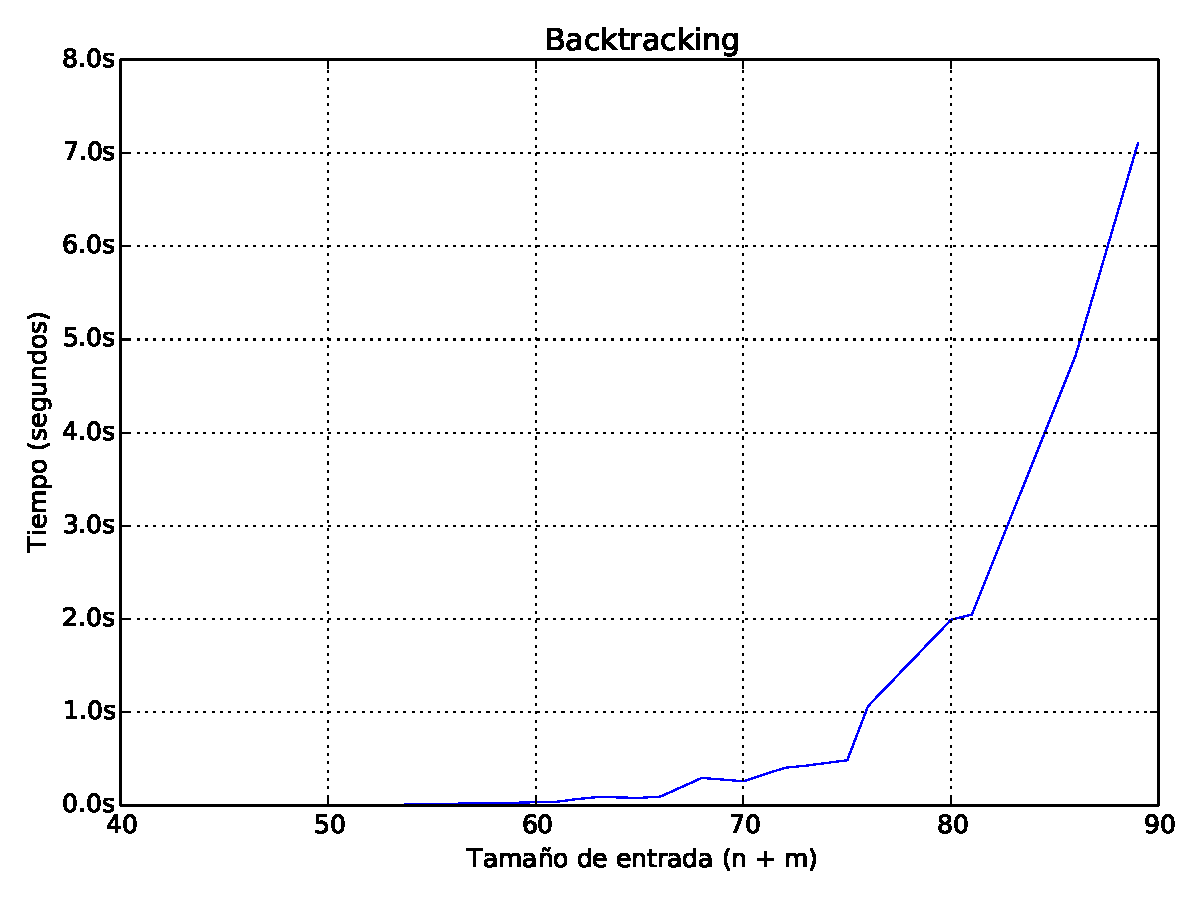
\includepdf[pages={1}]{imagenes/backtracking-aleatorio.pdf}
%
%Para tamaños de grafo menores que 40, los tiempos de ejecución fueron despreciables. Se puede apreciar el carácter exponencial del tiempo de
%ejecución de nuestro algoritmo en función del tamaño de entrada.

